\chapter{Covering the sphere with noncontextuality inequalities}\label{cha:Covering the sphere with noncontextuality inequalities}
This thesis will be based on the article by~\cite{PhysRevLett.101.020403} and the article by~\cite{Kochen1968The}. In the latter a set of 117 vectors are given. In this chapter it will be seen if it is possible to create pentagrams and pentagram inequalities using these vectors and the formulation given by~\cite{PhysRevLett.101.020403} such that the inequalities are violated for each direction on the sphere. 
If this is possible then they have presented an adequate test for hidden variables in spin 1 system.

Most of the details required to understand the following can be found in the previous introduction, mostly~\ref{sec:intro:Background of quantum mechanics:Operator formalism} and onward.
 
\newpage
\section{Evaluating the inequality}\label{sec:Covering the sphere with noncontextuality inequalities:Evaluating the inequality}
In this section an introduction to the inequality will be given. After this it shall be seen if a violation of the inequality can be found and what this means. 
\subsection{Choosing vectors}\label{subsec:Choosing vectors}
The operators are projection operators as in  appendix~\ref{cha:Calculations}. 
In the appendix several states/vectors are used, they are all given below as eigenvectors to these operators. These are all given in the article by ~\cite{Kochen1968The}. Not all of the vectors will produce pentagrams, however those that will can be written as the vectors below and rotations of these.
In a Carthesian Coordinate system the vectors after normalization are:
\\
\begin{equation*}
\begin{pmatrix}
0\\
0\\
1\\
\end{pmatrix}
,
\begin{pmatrix}
0\\
-\sin(\sfrac{\pi}{10})\\
\cos(\sfrac{\pi}{10})
\end{pmatrix}
,
\begin{pmatrix}
1\\
0\\
0\\
\end{pmatrix}
\end{equation*}
\begin{equation*}
\begin{pmatrix}
0\\
\cos(\sfrac{\pi}{10})\\
\sin(\sfrac{\pi}{10})\\
\end{pmatrix}
,
\begin{pmatrix}
-x\sqrt{1-x^2}*\cos(\sfrac{\pi}{10})\\
-\cos(\sfrac{\pi}{10})\sin(\sfrac{\pi}{10})*(1-x^2)\\
-\sin(\sfrac{\pi}{10})^2-x^2\cos(\sfrac{\pi}{10})^2\\
\end{pmatrix}
,
\begin{pmatrix}
x\sqrt{1-x^2}\cos(\sfrac{\pi}{10})\\
-\cos(\sfrac{\pi}{10})\sin(\sfrac{\pi}{10})(1-x^2)\\
-\sin(\sfrac{\pi}{10})^2-x^2\cos(\sfrac{\pi}{10})^2)\\
\end{pmatrix}
\end{equation*}
\begin{equation*}
\begin{pmatrix}
-\sqrt{1-x^2}\sin(\sfrac{\pi}{10})\\
-x\\
0\\
\end{pmatrix}
,
\begin{pmatrix}
-\sqrt{1-x^2}\sin(\sfrac{\pi}{10})\\
x\\
0\\
\end{pmatrix}
,
\begin{pmatrix}
-x\\
-\sqrt{1-x^2}\sin(\sfrac{\pi}{10})\\
\sqrt{1-x^2}\cos(\sfrac{\pi}{10})\\
\end{pmatrix}
,
\begin{pmatrix}
x\\
-\sqrt{1-x^2}\sin(\sfrac{\pi}{10})\\
\sqrt{1-x^2}\cos(\sfrac{\pi}{10})\\
\end{pmatrix}
\end{equation*}
Where x is given by:\\
\begin{equation*}
x=\sqrt{\frac{\sfrac{1}{2}}{10+2\sqrt{5}}(5+\sqrt{5}-\sqrt{-50+26\sqrt{5})}}
\end{equation*}
These vectors have been taken since they fulfil the properties in the appendix, such that they are pairwise orthogonal. They may look strange at first since if remembered from~\ref{Bloch Sphere} a phase shift of $\pi$, multiplication with $-1$ will not change anything. It should also be noted that from these 10 vectors the remaining 117 can be calculated by rotating these around the x-axis (first component axis) and rotating around the 111-axis, which comes from the article. To be able to understand and use these vectors in an easier way, they are also given below with 4 decimals.\\
\begin{equation*}
\begin{pmatrix}
0.0000\\
0.0000\\
1.0000\\
\end{pmatrix}
,
\begin{pmatrix}
-0.7071\\
-0.5172\\
-0.4822\\
\end{pmatrix}
,
\begin{pmatrix}
-0.5904\\
-0.8071\\
0.0000\\
\end{pmatrix}
,
\begin{pmatrix}
-0.5904\\
0.8071\\
0.0000\\
\end{pmatrix}
,
\begin{pmatrix}
0.7071\\
-0.5172\\
-0.4822\\
\end{pmatrix}
\end{equation*}
\begin{equation*}
\begin{pmatrix}
0.3892\\
-0.2847\\
0.8761\\
\end{pmatrix}
,
\begin{pmatrix}
-0.7071\\
-0.5172\\
-0.4822\\
\end{pmatrix}
,
\begin{pmatrix}
0.0000\\
0.9511\\
0.3090\\
\end{pmatrix}
,
\begin{pmatrix}
0.7071\\
-0.5172\\
-0.4822\\
\end{pmatrix}
,
\begin{pmatrix}
-0.3892\\
-0.2847\\
0.8761\\
\end{pmatrix}
\end{equation*}
Plotting these vectors, see figure~\ref{fig:penta1}, it can be seen that taking 5 of these vectors, still making sure that they are pairwise orthogonal, corresponding to commuting operators, it will produce a pentagram.
It is these pentagrams which will show the orthogonality relationships between the vectors. 
\subsection{Pentagram produced by the vectors}\label{subsec:Pentagram produced by the vectors}
If it is possible to take a set of five of these eigenvectors such that they are pairwise orthogonal then it will be possible to take eigenvectors to the operators that are orthogonal. This is to say that they commute and can be measured at the same time. The first pentagon chosen is the with the corners, which we will number as vectors/states:\\
\begin{equation*}
|\psi_1>=
\begin{pmatrix}
0.0000\\
0.0000\\
1.0000\\
\end{pmatrix}
,
|\psi_2>=
\begin{pmatrix}
0.5904\\
0.8071\\
0.0000\\
\end{pmatrix}
,
|\psi_3>=
\begin{pmatrix}
-0.7071\\
0.5172\\
0.4822\\
\end{pmatrix}
,
\end{equation*}
\begin{equation*}
|\psi_4>=
\begin{pmatrix}
0.7071\\
0.5172\\
0.4822\\
\end{pmatrix}
,
|\psi_5>=
\begin{pmatrix}
-0.5904\\
0.8071\\
0.0000\\
\end{pmatrix}
\end{equation*}
See the figure,~\ref{fig:penta1}, below where the vectors have been plotted and a pentagon plotted with the vectors as corners.
\begin{figure}[h!]
\begin{center}
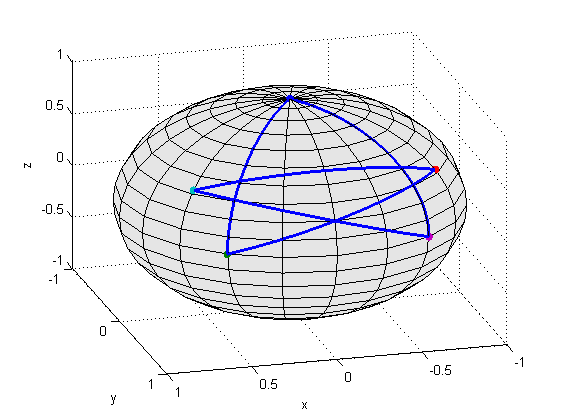
\includegraphics[scale=0.6]{penta1.png}
\caption{Pentagram 1 plotted on the Bloch sphere}
\label{fig:penta1}
\end{center}
\end{figure}
\\
Remember that a phase $\pi$ does not change the vectors. Now that the pentagon is understood, the inequality can be tackled. 
\subsection{Is the inequality violated?}
The inequality should be violated, as discussed in~\ref{sec:intro:Background of quantum mechanics:Ine}, somewhere inside of the pentagram.
In what area inside the pentagons is the inequality violated? 
From the calculations in \appendixref{cha:Calculations}, specifically~\ref{eq:Area1} the inequality~\eqref{eq:Inequality} is, using the vectors above, rewritten as the following:
\begin{dmath}\label{eq:Area}
5-4a_2^2-4(-0.5904a_0-0.8071a_1)^2-4(0.7071a_0-0.5172a_1-0.4822a_2)^2
-4(-0.7071a_0-0.5172a_1-0.4822a_2)^2-4(-0.5904a_0+0.8071a_1)^2 \geq -3
\end{dmath}
Since the only interesting solutions are those that exist on the spheres surface, that is to say that the vectors are normalized, $a_0^2+a_1^2+a_2^2=1$. These solutions can be simply visualized below. The question now arises if the violation inside or outside of the area?


Using any mathematical software to calculate the minimum value of the function of the left of the inequality, the minimum value is found as $-3.73559$ when $(a_0,a_1,a_2)$=(0,0.821597,-0.570069). This means that the inequality is violated atleast at this point which is \textbf{inside} the area. However it can be seen that the point is not inside our pentagram, this can be seen, either in the subsection above or below where the pentagram and area are plotted at the same time.
Now it must be seen if there exists an area inside the pentagon where the inequality is violated. 

\begin{figure}[h!]
\begin{center}
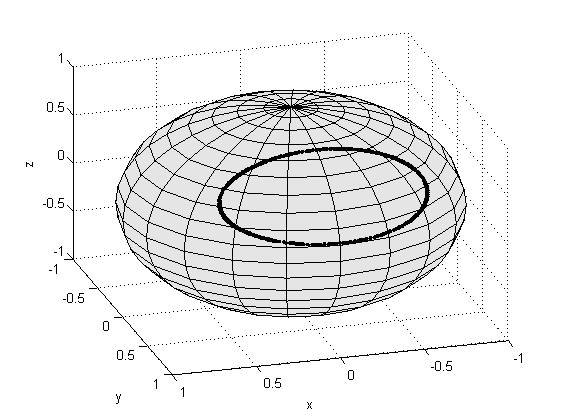
\includegraphics[scale=0.6]{ine1.png}
\caption{The first pentagram inequality plotted on the Bloch sphere}
\label{fig:ine1}
\end{center}
\end{figure}
\newpage
\subsection{Where is the inequality violated?}\label{subsec:Where is the inequality violated?}
By plotting the pentagram and the inequality in the same graph it can be seen where this area exists. See the simple plot below.
The dots are an outline of the area, in which the inequality is violated. As can be seen, there is an overlap between the pentagram and the inequality. There is also another area outside of the pentagram, this is excluded due to it being uninteresting since the quantum mechanical part excludes this area.
The observant will notice that since a phase shift of $\pi$ is unimportant there will of course be an identical area on the opposite side of the sphere. Everything that follows can be translated to that area by using a phase shift of $\pi$. There is a big overlap of the inequality and the pentagram, the parts that are not covered, can they be covered by other inequalities from other pentagrams? Otherwise there exists states that violate the pentagram inequality.
\begin{figure}[H]
\begin{center}
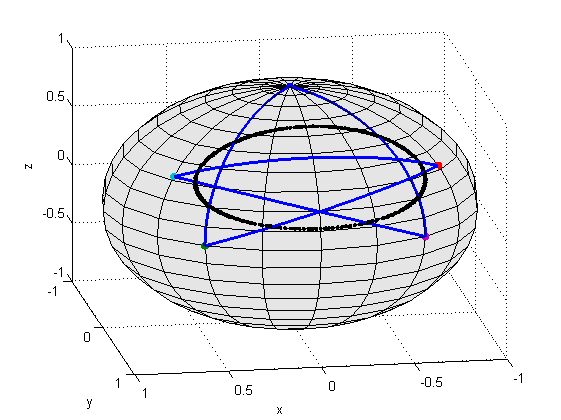
\includegraphics[scale=0.6]{sphere1ine.png}
\caption{Pentagram 1 with its inequality}
\end{center}
\end{figure}
\newpage
\section{Producing more pentagrams}\label{sec:Producing more pentagrams}
Starting with the simplest second pentagon. Given the vectors in~\subsectionref{subsec:Choosing vectors}, there is another pentagram that can be created, using the following vectors:
\begin{equation*}
|\psi2_1>=
\begin{pmatrix}
0.3892\\
-0.2847\\
0.8761\\
\end{pmatrix}
,
|\psi2_2>=
\begin{pmatrix}
0.0000\\
0.9511\\
0.3090\\
\end{pmatrix}
,
|\psi2_3>=
\begin{pmatrix}
-0.3892\\
-0.2847\\
0.8761\\
\end{pmatrix}
,
|\psi2_4>=
\begin{pmatrix}
0.7071\\
0.5172\\
0.4822\\
\end{pmatrix}
,
\end{equation*}
\begin{equation*}
|\psi2_5>=
\begin{pmatrix}
-0.7071\\
0.5172\\
0.4822\\
\end{pmatrix}
\end{equation*}
Using these vectors, the exact same procedure as in~\subsectionref{subsec:Pentagram produced by the vectors} is used. First a pentagon is produced, then the inequality is calculated with these vectors. See the pictures below 
\begin{figure}[H]
\begin{center}
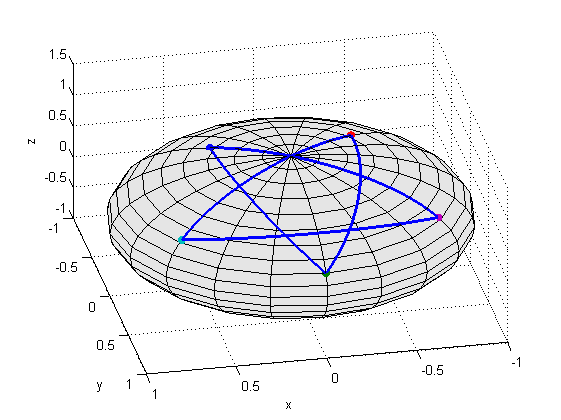
\includegraphics[scale=0.6]{penta2.png}
\caption{Pentagram 2 plotted on the Bloch sphere}
\label{fig:penta2}
\end{center}
\end{figure}
Now the inequality is plotted in the same picture.
\begin{figure}[H]
\begin{center}
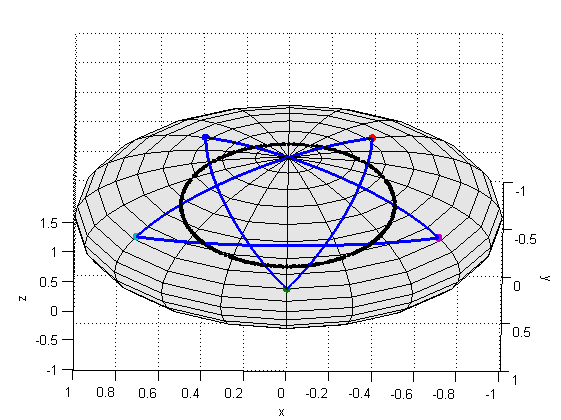
\includegraphics[scale=0.6]{sphere2ine.png}
\caption{Pentagram 2 with its inequality}
\end{center}
\end{figure}
\subsection{Where do the inequality areas overlap?}
How can the area be calculated?\\
Some of this is done in the appendix, by setting the equations for the two inequalities equal one can get out the intersecting points and from there calculate the area. However, this is quite tedious work and thus is done numerically, as most of the work above.
By plotting the two inequalities together it is shown that their areas do overlap, as seen below.
\begin{figure}[H]
\begin{center}
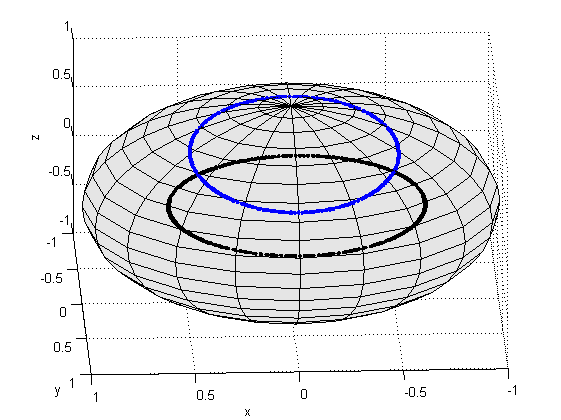
\includegraphics[scale=0.5]{ine12.png}
\caption{Pentagon 1 and 2 with their inequalities}
\end{center}
\end{figure}
To see if there is any part of the first pentagram not covered, the two inequalities are plotted over the first pentagram.
\begin{figure}[H]
\begin{center}
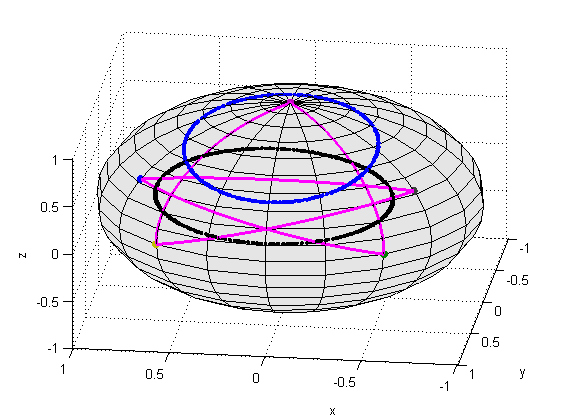
\includegraphics[scale=0.5]{penta1ine12.png}
\caption{Pentagon 1 with the inequality from 1 and 2}
\end{center}
\end{figure}
It can be seen in the later figure that four arms of the pentagram is uncovered by the pentagram, what must be remembered is that the interest lies at what part of the sphere is covered by the inequalities. This means that the only interest of the pentagram is to create the inequalities.


Now it must be seen what other pentagons can be created and what the inequality looks like in all of these.
One might think that this seem like a lot of unnecessary work, since it is the same inequality which should simply rotate with the pentagram. \textbf{This may however not be the case}, due to the fact that the inequality depends on the vectors used to produce the pentagram. This means that the inequality may not fill the sphere as expected. Also, the first rotation will be along an axis but not the second.
\newpage
\section{Producing even more pentagrams}
How can we produce more pentagrams? Simple take more vectors from~\cite{Kochen1968The} which can be represented as a rotation of our first vectors $18^\circ$ around the x-axis or around the vector: 
\begin{equation*}
\begin{pmatrix}
1\\
1\\
1\\
\end{pmatrix}
\end{equation*}
To start, rotate the inequalities that were discussed around the x-axis. If this produces a band that covers the entire sphere, and the point (1,1,1) then everything is done.
For simplicity, start with the rotation $18^\circ$ around the x-axis. For an easier plot, only the inequalities from the two first pentagrams are presented.
\begin{figure}[H]
\begin{center}
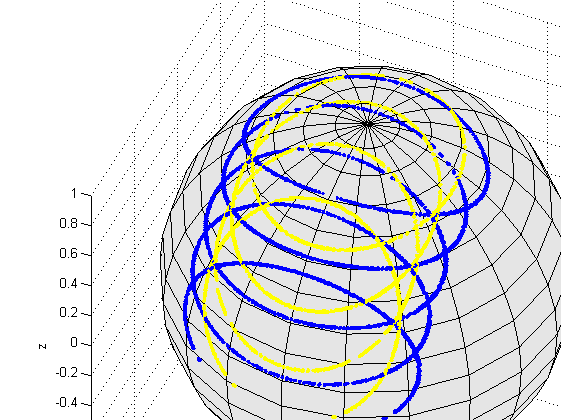
\includegraphics[scale=0.5]{ine12all.png}
\caption{The inequalities rotated around the x-axis.}
\label{fig:ine12all}
\end{center}
\end{figure}
It is seen that the the second inequalities are covered by the first, also the first inequalities create a band. Now the question is: Is the vector (1,1,1) inside the band? This is of importance since if it is then rotating the band around this point will cover the entire sphere. If not, then it must be seen if any rotated inequality can cover this point. First visually then using the formula from the appendix to calculate the inequality in the first pentagram. Remember the vectors given in~\ref{subsec:Pentagram produced by the vectors} which in the inequality produced~\eqref{eq:Area}. Inputting the vector (1,1,1) normalized with the factor $\frac{1}{\sqrt{3}}$ will result in $-3.0349 \geq -3$ which is false! Thus is it inside the inequality, see below.
\begin{figure}[H]
\begin{center}
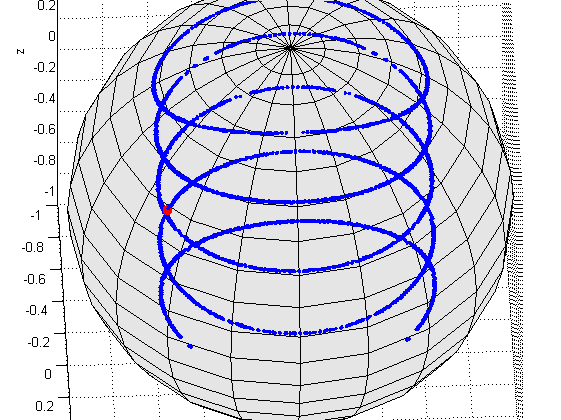
\includegraphics[scale=0.5]{ine12all111.png}
\caption{The inequalities rotated around the x-axis with the 111 vector plotted.}
\label{fig:ine12all111}
\end{center}
\end{figure}
Is the point inside the band produced by the rotated inequalities?
\subsection{Producing the band, is the point inside?}
How can the band be produced?
Calculate where the inequalities meet and see where the thinnest band is produced. By taking the scalar product between the overlap vectors an angle can be calculated, it is  this that will be used to create the band. Below a picture is presented of how three inequalities overlap and also where the vectors must be. 
\begin{figure}[H]
\begin{center}
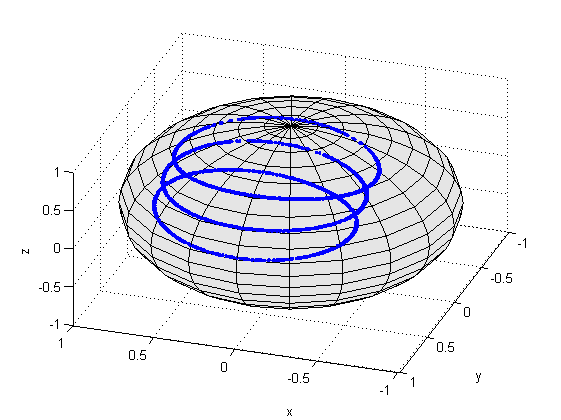
\includegraphics[scale=0.5]{overlap114.png}
\caption{Three inequalities plotted.}
\label{fig:overlap114}
\end{center}
\end{figure}
It is seen that the band is equally narrow both above and below. 
\begin{figure}[H]
\begin{center}
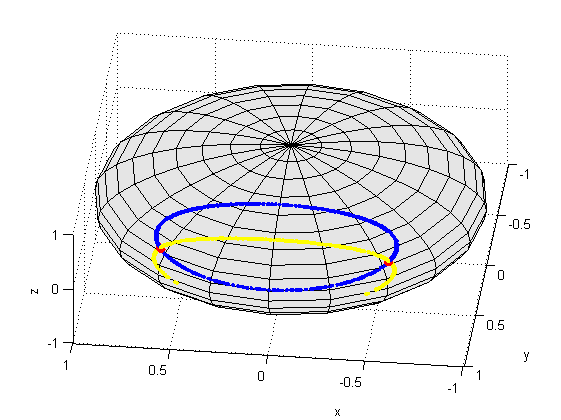
\includegraphics[scale=0.5]{band.png}
\caption{A plot of there limits to the band.}
\label{fig:band}
\end{center}
\end{figure}
Using the points above, one can draw small circles around the sphere. This is done by taking the x-coordinates from the intersection and plotting the following 
\begin{equation}
0.5812^2+y^2+z^2=1
\end{equation}
This is shown in the plot below with the point (1,1,1) visible.
\begin{figure}[H]
\begin{center}
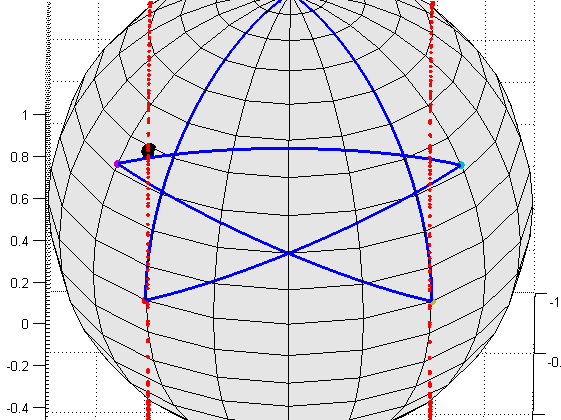
\includegraphics[scale=0.5]{completeband111big.png}
\caption{A plot of the band with the point (1,1,1)}
\label{fig:completeband}
\end{center}
\end{figure}
It can be seen above that the point (1,1,1) is inside the band. This is also seen from normalizing it and using the equation above (since $\frac{1}{\sqrt{3}}=0.5774<0.5812<1$
Since rotations are done around this point this means that the bands created by rotating the inequalities around will cover all points on the sphere if there is enough of an overlap between the rotated bands. 
\subsection{In the sphere covered?}\label{Is the sphere covered?}
As discussed in the previous subsection, if there is enough of an overlap between the rotated bands, then it is known that the sphere is covered and thus the goal of this thesis has been reached.
All three rotated bands can be seen in the figure below, here it is seen how the whole sphere is covered.
\begin{figure}[H]
\begin{center}
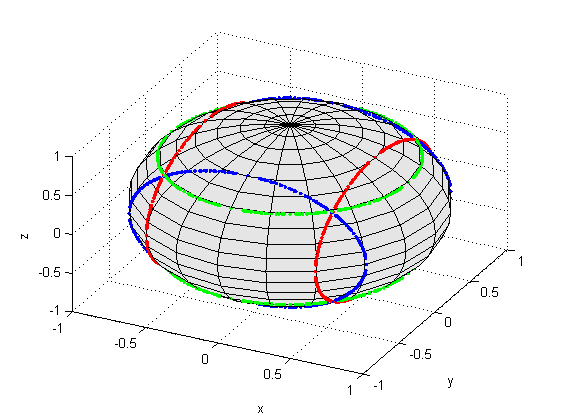
\includegraphics[scale=0.9]{coveredsphere.png}
\caption{The sphere covered with bands created by the inequalities}
\label{fig:coveredsphere}
\end{center}
\end{figure}
This means that the task has been complete, what conclusions can now be drawn from this thesis? 